\documentclass{standalone} 
\usepackage[tikz,plot,math]{forsyde}
\usepackage{forsyde-atom-docs}

\newcommand{\po}[1]{\underline{#1}}
\newcommand{\vbvec}{\rotatebox[origin=c]{-90}{$\langle$}}
\newcommand{\vevec}{\rotatebox[origin=c]{-90}{$\rangle$}}

\begin{document}
\begin{docimage}{example}
\begin{tikzpicture}[]
  \standard[process, moc=sdf, ni=2, no=2, f={$\lambda (a,b,c) (d,e) \rightarrow ((a+d,c+e),(b))$}, type=comb](p1){};
  \inputSY*[anchor=south west, shift={(-3cm, .2cm)}]  <p1.w1> {\po{1,2,3},\po{4,5,6},\po{7,8,9},...};
  \inputSY*[anchor=south west, shift={(-3cm,-.2cm)}]  <p1.w2> {\po{1,1},\po{1,1},\po{1,1},1};
  \outputSY*[yshift=.2cm]  <p1.e1> {\po{2,4},\po{5,7},\po{8,10}};
  \outputSY*[yshift=-.2cm]  <p1.e2> {\po{2},\po{5},\po{8}};
\end{tikzpicture}
\end{docimage}


\begin{docimage}{pattern-delay}
\begin{tikzpicture}[]
  \standard[process, moc=sdf, ni=1, no=1, f={$[0,0,0]$}, type=delay](p1){};
  \inputSY*  <p1.w1> {1,2,3,4,5};
  \outputSY*  <p1.e1> {0,0,0,1,2,3,4,5};
\end{tikzpicture}
\end{docimage} 

\begin{docimage}{pattern-delayp}
\begin{tikzpicture}[]
  \standard[process, moc=sdf, ni=2, no=1, type=delay'](p1){};
  \inputSY*[anchor=south west, shift={(-2cm, .2cm)}]  <p1.w1> {1,2,3,4,5};
  \inputSY*[anchor=south west, shift={(-2cm,-.2cm)}]  <p1.w2> {0,0,0};
  \outputSY*[]  <p1.e1> {0,0,0,1,2,3,4,5};
\end{tikzpicture}
\end{docimage} 

\begin{docimage}{pattern-comb}
\begin{tikzpicture}[]
  \standard[process, moc=sdf, ni=2, no=1, f={$\lambda (a,b,c) (d,e) \rightarrow ((a+d,c+e),(b))$}, type=comb](p1){};
  \inputSY*[anchor=south west, shift={(-2cm, .2cm)}]  <p1.w1> {\po{1,2,3},\po{4,5,6},\po{7,8,9},...};
  \inputSY*[anchor=south west, shift={(-2cm,-.2cm)}]  <p1.w2> {\po{1,1},\po{1,1},\po{1,1},1};
  \outputSY*[]  <p1.e1> {\po{2,4},\po{5,7},\po{8,10}};
\end{tikzpicture}
\end{docimage} 

\begin{docimage}{pattern-reconfig}
\begin{tikzpicture}[]
  \standard[process, moc=sdf, ni=2, no=1, type=reconfig](p1){};
  \inputSY*[anchor=south west, shift={(-4cm, .2cm)}]  <p1.w1> {$\Sigma,\max,\Sigma,\max,\Sigma,\max,\Sigma$};
  \inputSY*[anchor=south west, shift={(-4cm,-.2cm)}]  <p1.w2> {\po{1,2,3,4},\po{5,6,7,8},...};
  \outputSY*  <p1.e1> {\po{10},\po{8},\po{42},\po{16},\po{74},\po{24},\po{106}};
\end{tikzpicture}
\end{docimage} 


\begin{docimage}{pattern-constant}
\begin{tikzpicture}[]
  \standard[process, moc=sdf, no=2, f={$((1,2,3),(2,1))$}, type=constant](p1){};
  \outputSY*[yshift=.2cm]  <p1.e1> {\po{1,2,3},\po{1,2,3},...};
  \outputSY*[yshift=-.2cm] <p1.e2> {\po{2,1},\po{2,1},\po{2,1},...};
\end{tikzpicture}
\end{docimage} 

\begin{docimage}{pattern-generate}
\begin{tikzpicture}[]
  \standard[process, moc=sdf, no=2,
    f={$\lambda\ a\ b \rightarrow ((\Sigma a, \Sigma a),(\Sigma b, \Sigma b, \Sigma b))$;$(1,1),(2,2,2)$},
    type=generate](p1){};
  \outputSY*[yshift=.2cm]  <p1.e1> {\po{1,1},\po{2,2},\po{4,4},8,...};
  \outputSY*[yshift=-.2cm] <p1.e2> {\po{2,2,2},\po{6,6,6},18,18,...};
\end{tikzpicture}
\end{docimage} 

\begin{docimage}{pattern-state}
\begin{tikzpicture}[]
  \standard[process, moc=sdf, f={$\lambda(a)(b,c) \rightarrow (a+b+c)$;$(1)$}, type=state](p1){};
  \inputSY*  <p1.west> {\po{1,2},\po{3,4},\po{5,6},7};
  \outputSY* <p1.east> {\po{1},\po{4},\po{11},\po{22}};
\end{tikzpicture}
\end{docimage} 

\begin{docimage}{pattern-stated}
\begin{tikzpicture}[]
  \standard[process, moc=sdf, f={$\lambda(a)(b,c) \rightarrow (a+b+c)$;$(1)$}, type=stated](p1){};
  \inputSY*  <p1.west> {\po{1,2},\po{3,4},\po{5,6},7};
  \outputSY* <p1.east> {\po{4},\po{11},\po{22}};
\end{tikzpicture}
\end{docimage}

\begin{docimage}{pattern-moore}
\begin{tikzpicture}[]
  \standard[process, moc=sdf, f={$\lambda(a)(b,c) \rightarrow (a+b+c)$;$\lambda(a) \rightarrow (a+1,a\times 2)$;$(1)$}, type=moore](p1){};
  \inputSY*  <p1.west> {\po{1,2},\po{3,4},\po{5,6},7};
  \outputSY* <p1.east> {\po{2,2},\po{5,8},\po{12,22},\po{23,44}};
\end{tikzpicture}
\end{docimage}

\begin{docimage}{pattern-mealy}
\begin{tikzpicture}[]
  \standard[process, moc=sdf, f={$\lambda(a)(b,c) \rightarrow (a+b+c)$;$\lambda(a)(b) \rightarrow (a+b,a\times b)$;$(1)$}, type=mealy](p1){};
  \inputSY*  <p1.west> {\po{\po{1},\po{2}},\po{\po{3},4},\po{5,6},7};
  \outputSY* <p1.east> {\po{2,1},\po{6,8},\po{14,33},\po{26,88}};
\end{tikzpicture}
\end{docimage}

\begin{docimage}{tosy}
\begin{tikzpicture}[]
  \standard[process, ni=1, moc=sdf, type=toSY](p1){};
  \inputSY*  <p1.w1> {1,2,3,4,5};
  \outputSY* <p1.e1> {1,2,3,4,5};
\end{tikzpicture}
\end{docimage}

\begin{docimage}{zipx}
\begin{tikzpicture}[]\scriptsize
  \trans[transition=s1v1, rotate shape=180, ni=4, moc=sdf, type=zipx](p1){};
  \node[shift={(-3, .35)}, anchor=south west] (p1w1) at (p1.w1) {\po{1,2},\po{3,4},5};
  \node[shift={(-3, .15)}, anchor=south west] (p1w2) at (p1.w2) {\po{1},\po{2},3,4,5};
  \node[shift={(-3,-.15)}, anchor=south west] (p1w3) at (p1.w3) {\po{11,12},\po{13,14},15};
  \node[shift={(-3,-.35)}, anchor=south west] (p1w4) at (p1.w4) {\po{11},\po{12},13,14,15};
  \node[anchor=south west, xshift=1cm] (p1e1) at (p1.e1) {%
    $\begin{array}{cc}
      \vbvec & \vbvec \\
      1  & 3  \\
      2  & 4  \\
      1  & 2  \\
      11 & 13 \\
      12 & 14 \\
      11 & 12 \\
      \vevec & \vevec
    \end{array}$
  };
  \path[s,->, -|-=.9]
  (p1w1.south west) edge (p1.w1)
  (p1w2.south west) edge (p1.w2)
  (p1w3.south west) edge (p1.w3)
  (p1w4.south west) edge (p1.w4)
  (p1.e1) edge (p1e1.south east);
\end{tikzpicture}
\end{docimage}

\begin{docimage}{unzipx}
\begin{tikzpicture}[]\scriptsize
  \trans[transition=s1v1, no=4, moc=sdf, type=zipx](p1){};
  \node[shift={(3, .35)}, anchor=south east] (p1e1) at (p1.e1) {\po{1,2},\po{3,4}};
  \node[shift={(3, .15)}, anchor=south east] (p1e2) at (p1.e2) {\po{1},\po{2}};
  \node[shift={(3,-.15)}, anchor=south east] (p1e3) at (p1.e3) {\po{11,12},\po{13,14}};
  \node[shift={(3,-.35)}, anchor=south east] (p1e4) at (p1.e4) {\po{11},\po{12}};
  \node[anchor=south east, xshift=-1cm] (p1w1) at (p1.w1) {%
    $\begin{array}{cc}
      \vbvec & \vbvec \\
      1  & 3  \\
      2  & 4  \\
      1  & 2  \\
      11 & 13 \\
      12 & 14 \\
      11 & 12 \\
      \vevec & \vevec
    \end{array}$
  };
  \path[s,<-, -|-=.9]
  (p1e1.south east) edge (p1.e1)
  (p1e2.south east) edge (p1.e2)
  (p1e3.south east) edge (p1.e3)
  (p1e4.south east) edge (p1.e4)
  (p1.w1) edge (p1w1.south west);
\end{tikzpicture}
\end{docimage}


\end{document}

%%% Local Variables:
%%% TeX-command-default: "Make"
%%% mode: latex
%%% TeX-master: t
%%% End:
